\documentclass[12pt, a4paper]{scrbook}
\usepackage[utf8]{inputenc}
\usepackage{csquotes}
\usepackage[german]{babel}
\usepackage{hyperref}
\usepackage[onehalfspacing]{setspace}
\usepackage{geometry}
\usepackage{color}
\usepackage{listings}
\usepackage{graphicx}
\usepackage{acronym}
\usepackage[backend=biber,
bibstyle=alphabetic, 
citestyle=authortitle,
natbib=true, 
hyperref=true,
]{biblatex}
\addbibresource{lit.bib} 
\setcounter{secnumdepth}{4}
\setcounter{tocdepth}{4}
\geometry{
left=2.5cm,
right=2.5cm,
top=2.5cm,
bottom=2.5cm,
bindingoffset=5mm,
}
\pagestyle{empty}
\begin{document}
%\documentclass[titlepage, 12pt]{scrbook}
%\usepackage[utf8]{inputenc}
%\usepackage[german]{babel}
%\usepackage{uarial}
%\usepackage{color}
%\renewcommand{\familydefault}{\sfdefault}
%\usepackage{fancyhdr}
%\usepackage{graphicx}
%\pagestyle{empty}
%\begin{document}
\begin{titlepage}
	\begin{flushleft}
	\begin{figure}
		\hspace*{-0,5cm}
		
\includegraphics[scale=0.25]{Bilder/DHBW_logo.jpg} \hspace*{5cm}
		
\includegraphics[scale=0.25]{Bilder/Atos_logo.png}
	\end{figure}
	\end{flushleft}
	\vspace*{-0.6cm}
	\begin{center}
	\textcolor{red}{Titel der großen Studienarbeit} \par \vspace*{0,5cm}
	Projektarbeit \par \vspace*{2cm}
	des Studienganges \textcolor{red}{Angewandte Informatik / Betriebliches Informationsmanagement}
	an der Dualen Hochschule Baden-Württemberg Mannheim \par \vspace*{1cm}
	von \par \vspace*{0,5cm}
	\textcolor{red}{Maximilian Ludwig, Kevin Wrona, Fabian Brandmüller} \par \vspace*{1cm}
	\today \par \vspace*{2cm}
	\begin{tabular}{l@{\hspace{3cm}}r}
		Bearbeitungszeitraum & \textcolor{red}{23.09.2019 - 20.04.2019} \\
		Betreuer der DHBW & \textcolor{red}{Eckhard Kruse} \\[1cm] 
	\end{tabular}
	\end{center}
\end{titlepage}
%\end{document}
\setlength{\parindent}{0em} 
\renewcommand\thechapter{\Roman{chapter}}
\pagenumbering{Roman}
\let\cleardoublepage\relax
\section*{Erklärung}
Ich versichere hiermit, dass ich meine Projektarbeit mit dem Thema: ''Titel der großen Studienarbeit'' selbstständig verfasst und keine anderen als die angegeben Quellen und Hilfsmittel benutzt
habe.
\newline
\newline
\newline
\newline
---------------------------------------------       ------------------------------------------ \newline
Ort	\hspace{2cm}		Datum\hspace{3,5 cm}				    Unterschrift
\newpage
\section*{Abstract}


\newpage
\begingroup
\renewcommand*{\chapterpagestyle}{empty}
\pagestyle{empty}
\tableofcontents
\listoffigures
\section*{Abkürzungen}
\begin{acronym}[Bash]
% \acro{VCS}{Version Control System}
\end{acronym}
\endgroup
\newpage
\pagestyle{plain}
\setcounter{page}{1}
\chapter{Einleitung}
''Several researchers have stated that facial expression recognition appears to play one of the most important roles in human communication'' 
\footcite[Vgl.][1]{FaceRec}
Dieses Zitat von Katherine B. Leeland gibt einen Einblick in die Relevanz der Emotionserkennung für den Menschen. Fragen zu dieser Thematik stellen sich allerdings nicht erst seit Beginn der Digitalisierung. Bereits Darwin
fragte sich, ob von den Gesichtsausdrücken einer Person nicht auch der Emotionale Zustand abgeleitet werden kann.
\footcite[Vgl.][2]{FaceRec}
Einen solchen Zustand von einem Mitmenschen abzulesen ist jedoch nicht nicht leicht zu realisieren. Bereits durch kleine Änderungen in der Mimik werden verschiedene Emotionen ausgedrückt. Zum Beispiel indem eine Person die Lippen zusammen presst und die Augen zusammen kneift bei Wut, oder die Mundwinkel nach unten gezogen werden bei Trauer.
\footcite[Vgl.][249]{HandbookFaceRec}
Durch derartige Ausdrücke können Emotionen wie Wut oder Trauer Ausdruck gewinnen.
Emotionserkennungssoftware gibt es bereits und wird auch in der Wirtschaft eingesetzt. Die Anwendungsgebiete reichen dabei von Jobinterviews, in denen analysiert wird in wie weit die Bewerber für
den jeweiligen Job geeignet sind, 
\footcite[Vgl.][]{mixedArticle}
bis hin zur Automobilindustrie. Dort wird mittels geeigneter Sensorik versucht die Emotion und somit der physiologische Zustand des Autofahrers zu analysieren.
\footcite[Vgl.][Herausforderung]{Frauenhofer}
Diese Daten legen den Grundbaustein für Warnsysteme, welche den Fahrer darauf hinweisen können, dass sein Zustand ungeeignet zum Betrieb eines Kraftfahrzeugs ist. Jedoch werden
solche Einsatzszenarien auch durchaus kontrovers diskutiert. Auf Kritik stößt unter anderem dass die sogenannten ''Basisemotionen'', die verwendet werden um den KIs Emotionserkennung
beizubringen, selbst umstritten sind.
\footcite[Vgl.][]{SZ}
Aber auch ethische bedenken werden zunehmend geäußert, vor allem bezüglich der Anwendungsgebiete. Denn je nach Emotion die erkannt werden soll, liegt die Fehlerrate sehr hoch. So hat das
Frauenhofer Institut, welches an Einsatzgebieten von Emotionserkennung in Fahrzeugen arbeitet, festgestellt, dass eine Emotionserkennung je nach Zielemotion eine Vorhersagekraft zwischen 6 und
95\% haben kann.
\footcite[Vgl.][Ergebnis]{Frauenhofer}
Diese negativen Aspekte treffen jedoch nur teilweise auf das hier behandelte Forschungsprojekt zu, wie im Folgenden dargelegt werden soll:
Es werden in dieser Arbeit die Basisemotionen als Referenz herangezogen. Dies ist notwendig, da die Alternativen Verfahrensweisen zur Ermittlung
der Emotion eines Individuums nicht praktikabel für den Use Case dieser Arbeit wären. Eine erweiterte Betrachtung der Alternativen findet sich in Kapitel II. Des weiteren ist diese
Studienarbeit kein wissenschaftliches Werk über die psychologischen Emotionen die hinter verschiedenen Gesichtsausdrücken stehen, auch wenn sie dies indirekt thematisiert. In dieser Arbeit geht es darum die
These zu verifizieren oder zu widerlegen, ob es möglich ist mit einer künstlichen Intelligenz zu erkennen, in wie weit ein Pokerface einer Person anhand dessen Gesichtsausdruck abgelesen werden
kann. Diese Aufgabe hat also nicht den Anspruch eine Emotion korrekt vorherzusagen, sondern vorherzusagen wann keine Emotion vorliegt. Denn Ein Pokerface wird im Allgemeinen als ein
emotionsloser Gesichtsausdruck definiert. Dies impliziert, dass eine Person mit Pokerface keine Emotion zu erkennen gibt. Daher könnte bei einer nicht messbaren, oder neutralen Emotion ein
Pokerface vorliegen. Dies mittels KI zu testen und einen sogenannten ''Pokerface Detektor'' zu entwickeln ist folglich Ziel dieser Arbeit. Mit diesem Pokerface Detektor sind verschiedenste
Einsatzmöglichkeiten in der Praxis denkbar. Diese haben eine gewisse Schnittmenge mit denen von ''normaler'' Emotionserkennungssoftware, jedoch gibt es auch einige weitere. Im Folgenden werden
einige mögliche Szenarien expliziert:
\begin{itemize}
	\item{Polizeiverhöre}
\end{itemize}
Es ist denkbar, dass der zu entwickelnde Detektor bei Polizeiverhören eingesetzt werden könnte. Hierdurch könnten Beamte die Verwendung eines Pokerfaces durch den Beschuldigten erkennen, welches auf eine Lüge hinweisen könnte. Neben der gebräuchlichen Verwendung eines Lügendetektors wäre der Einsatz der in dieser Arbeit erstellten Lösung eine kostengünstige Variante.
\begin{itemize}
	\item{Gerichtsverhandlungen}
\end{itemize}
Das zweite Einsatzgebiet ist ähnlich zu dem ersten. Bei Gerichtsverhandlungen gelten die gleichen Voraussetzungen wie bei einem Verhör der Polizei. Zwar müssen die Vorgeladenen eine
eidesstattliche Erklärung abgeben nur die Wahrheit zu sagen, jedoch ist zu bezweifeln ob dies auch der Fall ist.
Nun soll nicht der Eindruck entstehen dass das hier gebaute Werkzeug ein Lügendetektor ist. Es ist ebenfalls nicht möglich, dass von einem Pokerface immer auf eine Lüge geschlossen werden kann.
Jedoch ist ein Pokerface ein Zeichen dafür, dass sich diese Person ihren emotionalen Zustand nicht anmerken lassen möchte. Und dies wiederum deutet eher daraufhin dass die Person nicht die
Wahrheit sagt oder nur teilweise.
Abgesehen von Einsatzgebieten die zur Entlarvung von Lügen führen, kann auch ein klassisches Szenario verwendet werden:
\begin{itemize}
	\item{Pokerspiel}
\end{itemize}
Es ist anzunehmen, dass der erste Begriff der mit dem Wort Pokerface in Verbindung gebracht wird, das Pokerspiel selber ist. Und auch in diesem kann ein Pokerface Detektor nützlich sein. So kann
ein Mitspieler zum Beispiel mittels einer Kamera das Gesicht des Gegenübers scannen und analysieren ob ein Pokerface vorliegt oder nicht, und dementsprechend agieren.
Nachdem verschiedene Anwendungsszenarien beleuchtet wurden wird im Folgenden die konkrete Forschungsfrage beleuchtet.
%Irgendwas vergessen?
\section{Aufgabenstellung}
 Das Projekt selber wird an der DHBW in Mannheim durchgeführt und von Prof. Dr. Erckhard Kruse betreut.
 Wie eingangs erwähnt soll mittels künstlicher Intelligenz ein Pokerface erkannt werden. 
Zur Umsetzung dieser Aufgabe wird eine Bilderkennungssoftware angefertigt, welches ein übermitteltes Bild nach vorhandenen Emotionen analysiert. Sollte keine Emotion durch die Software erkannt werden, wird dem Anwender das Vorhandensein eines Pokerfaces zurück gegeben. Ein konkretes Einsatzgebiet nach Abschluss der Entwicklung ist nicht
vorgesehen, da es sich um ein Forschungsprojekt handelt. Jedoch sind wie bereits in der Einleitung beschrieben einige verschiedene Einsatzmöglichkeiten denkbar, an die das Werkzeug leicht angepasst werden kann.

%\section{DevOps}
%\begin{figure}
%\includegraphics[width=\linewidth]{Bilder/DevOps-LifeCycle-Features-Naresh-IT.png}
%\caption{ DevOps Lifecyle \newline Quelle: https://nareshit.com/wp-content/uploads/2018/09/DevOps-LifeCycle-Features-Naresh-IT.png }
%\label{fig:Devops-Lifecycle}
%\end{figure}


\let\cleardoublepage\relax
\chapter{Theorie}
Technologien todo:
\begin{itemize}

\item Poker erklären (Wenn wir Poker als testusecase benutzen)
\end{itemize}

\section{Stand der Technik}
In diesem Abschnitt soll der aktuelle Forschungs- und Entwicklungsstand im Bereich Emotionserkennung thematisiert werden. Jedoch muss dafür erst einmal eine Unterscheidung der Begrifflichkeiten
Emotionserkennung und Gesichtserkennung erfolgen, da beide gebiete Überschneidungen haben, jedoch inhaltlich und von ihren Zielen verschieden sind.

\subsection{Geischtserkennung}
\begin{itemize}
\item use cases von Gesichtserkennung
\item Grenzen der Gesichtserkennung
\item Ausblick in der Gesichtserkennung
\end{itemize}

Gesichtserkennung ist eine Disziplin der Informatik in der es darum geht Gesichter wieder zu erkennen, und gegebenanfalls verschiedenen Personen zuzuordnen. Dabei lässt sich der Prozess der
Gesichtserkennung in vier Phasen einteilen, Face ''detection'', ''alignment'', ''feature extraction'' und ''matching''.
\footcite[Vgl. ][2]{HandbookFaceRec}
\begin{figure}
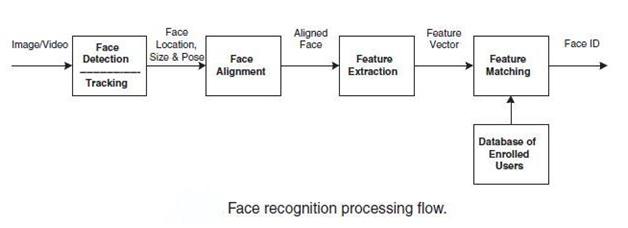
\includegraphics[width=\linewidth]{Bilder/FaceRecognition.png}
\caption{ Phasen der Gesichtserkennung \newline Quelle: https://alitarhini.files.wordpress.com/2010/12/untitled1.png }
\label{fig:Face Recognition}
\end{figure}
Die Detection Phase ist dafür verantwortlich um zu erkennen ob Gesichter vorhanden sind in einem Bild, oder aber Video.
\footcite[Vgl. ][2]{HandbookFaceRec}
In der darauffolgenden Alignment Phase hingegen wird die Lokalisierung der Gesichter genauer, indem Gesichtskomponenten wie Augen, Augenbrauen, oder die Nase genauer lokalisiert werden. Dabei
wird das Bild oder Video ebenfalls normalisiert, indem z.B. die Bildbeleuchtung angepasst wird.
 \footcite[Vgl. ][2]{HandbookFaceRec}
In der Feature extraction hingegen werden die verschiedenen Gesichtskomponenten wie Augen, Nase, Mund, dem Bild oder Video entnommen. Dies ist ein wichtiger Schritt für weitere Prozesse wie
Eye Tracking oder Face Tracking. Alternativ kann sogar eine bestimmte Person anhand der extrahierten Merkmale erkannt werden.
\footcite[Vgl. ][Abstract]{IEEE}
In der letzten Phase, dem Matching, geht es darum die gewonnen Daten mit den in der Datenbank vorhandenen Gesichtern abzugleichen. Wenn eine genügende Übereinstimmung gefunden wurde, wird ein
Match mit einer Person ausgegeben.
  \footcite[Vgl. ][3]{HandbookFaceRec}
Die Anwendungsgebiete von Software die Gesichtserkennung ermöglicht ist mannigfaltig. Sie reicht von Applikationen die ein Gerät wie ein Smartphone entsperren, wenn das Gesicht des Besitzers als
Match ausgegeben wurde, bis hin zur Anwendung in Verbrechensbekämpfung. In jedem dieser Szenarien wird dabei der oben beschriebene Ablauf durchgegangen, und abhängig vom zu liefernden Ergebnis
eine Abschlussaktion vorgenommen.
 
\subsection{Emotionserkennung}

\begin{itemize}
\item was ist Emotionserkennung
\item usecase für emotion recognition
\item Ausblick und Kontroverse
\end{itemize}

 
\subsection{Gemeinsamkeiten und Unterschiede}
\begin{itemize}
\item Gemeinsamkeiten und Unterschiede in Anwendungsgebieten
\item formalen Aspekten
\end{itemize}

\section{Emotionen}

\begin{itemize}
\item Def. von Emotionen
\end{itemize}

In diesem Unterkapitel nun sollen Emotionen an sich thematisiert werden, da diese maßgeblich sind für das zu entwickelnde Tool. Grundsätzlich gibt es  verschieden Ansätze Emotionen zu
definieren und einzuteilen. Eine Variante ist dabei die eingangs erwähnte, nicht ganz unumstrittene Einteilung in Basisemotionen. Eine gängige Einteilung ist dabei die verschiedenen
Emotionen in acht Bereiche einzuteilen. Diese Einteilung wurden 1984 von Plutchik postuliert und beinhaltet die Emotionskategorien Angst, Wut, Freude, Trauer, Akzeptanz, Ekel, Erwartung und
Überraschung.
\footcite[Vgl. ][3]{FaceRec}
Jedoch ist dies nicht die einzige mögliche Einteilung. Als weiteres Beispiel teilte MacLean die Emotionen in lediglich sechs Kategorien ein, welche da wären: Verlangen, Wut, Angst,
Niedergeschlagenheit, Freude und Zuneigung.
\footcite[Vgl. ][3]{FaceRec}
Wie sich bereits an den beiden Beispielen zeigt, geht die Meinungen der Forscher dabei  stark auseinander, welche und wie viele Emotionen zu den sogenannten ''Basis Emotionen'' gehören. In
dieser Arbeit werden die Emotionen in sechs Kategorien eingeteilt, in Wut, Trauer, Freude, Ekel, Überraschung und Neutral. Diese Einteilung entspricht an sich keiner gängigen Einteilung, jedoch
wurde diese aus den folgenden Gründen gewählt: \newline
Die hier genannten Emotionen lassen sich gut anhand von Bildern erlernen, da diese zum Teil komplementär und somit eindeutig sind. Es ist aber auch einfacher Testdatensätze zu bekommen für ein
freudiges Gesicht, oder ein überraschtes, als ein Gesicht mit dem emotionalen Ausdruck Akzeptanz. Des Weiteren wurde der Ausdruck ''Neutral'' hinzugefügt. Neutral repräsentiert ein emotionsloses
Gesicht, und somit nach Definition einem Pokerface. Zudem sind die gewählten Emotionen häufig bei dem Test Usecase dieser Arbeit anzutreffen, dem Texas Holdem Poker.

\section{Python}
\begin{itemize}
\item Python (Als ganzes warum Python, Libraries erklären, warum python verwendet wurde und state of the art ist
\item Tensorflow und Kreas wenn wir es verwenden aber auch wenn wir es nicht machen
\item verwendeter Datensatz
\item CNN --> Wie arbeitet die KI bei Gesichtserkennung ?
\end{itemize}

\section{Alternative Ansätze}
In diesem Abschnitt nun werden noch verschiedene alternative Ansätze dargestellt und expliziert warum sich gegen diese, und für die bereits genannten Verfahrensweisen entschieden wurde.
\subsection{Emotionserkennung}
Dieses Unterkapitel beschäftigt sich mit alternativen Ansätzen zu den bereits explizierten Basisemotionen. Diese sind wie bereits erwähnt umstritten, was die Frage zulässt warum diese überhaupt
verwendet werden sollten. Ein weiterer kreativer Ansatz zur Erkennung von Emotionen wäre die Analyse der Stimmlage.
Dieser Ansatz beruft sich darauf, dass das Sprachzentrum eines Menschen einer der wichtigsten Aspekte der Kommunikation und somit auch der Preisgabe von Informationen über den emotionalen Zustand eines Individuums ist.
\footcite[Vgl. ][Abstract]{EmotionInSpeech}
Dieser Ansatz ist jedoch nicht zielführend, da hier hauptsächlich die Stimme analysiert wird. Von einer Stimme kann nun auf eine Emotion geschlossen werden. Für den Usecase ist dieser Ansatz allerdings ungeeignet, aus folgenden Gründen:
\newline
Es kann möglich sein eine Emotion anhand der Sprache zu erkennen. Das Äquivalent eines Pokerfaces wäre dementsprechend eine neutrale Stimmlage, welche keine Emotionen suggeriert. Nun kann aber keine Aussage getroffen werden aus welchen Gründen eine Person neutral spricht. Es könnte von einem Pokerface stammen, oder einer monotonen Sprechweise, oder einen gelangweilten Gemütszustand. Dies ist nicht eindeutig identifizierbar. Gleiches könnte nicht über ein neutrales Gesicht gesagt werden, da dies gemeinhin als Pokerface bezeichnet wird. %Spricht das nicht auch gegen unser Vorgehen?
Ein weitere Ansatz wäre die Analyse der derzeit vernommenen Musik. Diese kann einem bestimmten Gemütszustand zugesprochen werden, welches auf eine aktuelle Emotion übertragbar ist.
\footcite[Vgl.][1]{MusicEmotion}
 Ziel dieses Forschungszweiges ist es daher die hinter Liedern oder Klängen stehenden Emotionen zu ermitteln und diese entsprechend zu kategorisieren.
Dieser Ansatz erscheint zunächst durchaus interessant, hat jedoch genauso Nachteile wie die Analyse von Emotionen anhand von Bildern die Basisemotionen zeigen. %Spricht wieder gegen unser Vorgehen
Dieser liegt hier unter anderem in der Genauigkeit der Analysen. So z.B. lieferte ein Testprojekt an der Russichen HSE (Higher School of Economics) das Ergebnis von einer maximalen Genauigkeit von 71\%.
\footcite[Vgl. ][Abstract]{EmotionInSound}
In dem Versuchsaufbau wurden Spektrogramme von Klangfragmenten ausgewertet und versucht mittels Neuronalen Netzen eine Klassifikation der hinter dem Klang liegenden Emotion zu erreichen.
\footcite[Vgl. ][Abstract]{EmotionInSound}
Der generelle Ansatz anhand von Musik die Emotion eines Individuums abzulesen ist zwar praktikabel und von dem Versuchsaufbau auch vergleichbar zu dem Ansatz bereits gelabelte Bilder zu verwenden. Jedoch lässt sich auf diese Weise aus zwei Gründen nicht die eigentliche Zielaufgabenstellung ableiten, das Erkennen eines Pokerfaces. Zum einen handelt es sich in dieser Arbeit um eine visuelle Problemstellung, in welcher das Erkennen des Gemütszustandes anhand des Gesichtsausdruckes erkannt werden soll, also einem vorhandenen bzw. nicht vorhandenen Pokerface. Zum anderen würde die Analyse von Musik einen Rückschluss auf den allgemeinen Gemütszustand des Betroffenen folgern und nicht eine kurzzeitige Stimmungsschwankung aufgrund beispielsweise eines schlechten Blattes, wie in diesem Usecase.
\let\cleardoublepage\relax
\newpage
\chapter{Methode}

Als vorgehen könnten wir sagen dass wir die neuen Algorithmen oder Daten beim Poker teste, das wäre Lustig und ein Use case der Sinn macht. Mehr als sich stupide vor die Kamera zu setzen.

Diese Arbeit soll methodisch mit der MoSCoW Priorisierung bearbeitet werden. Diese Art der Priorisierung teilt die zu bearbeitenden Anforderungen in vier Kategorien ein:
\footcite[vgl.][90]{Projektmanagement}
\begin{itemize}
\item Must - Core Anforderungen die unbedingt umgesetzt werden müssen
\item Should - Anforderungen die ebenfalls umgesetzt werden müssen, jedoch um Nachhinein noch durch Change Request verändert werden können.
\item Could - Anforderungen die Nach den Must und Should Anforderungen umgesetzt werden sollen, sofern noch Ressourcen und Zeit vorhanden sind um diese zu bearbeiten
\item Won't - Anforderungen die nicht in diesem Projekt bzw. Release erfolgen, jedoch in einer zukünftigen Version bearbeitet werden sollen. 
\end{itemize}


\begin{itemize}
\item Must
\begin{itemize}
\item placeholder
\end{itemize}
\item Should
\begin{itemize}
\item placeholder
\end{itemize}
\item Could
\begin{itemize}
\item placeholder
\end{itemize}
\item Won't
\begin{itemize}
\item placeholder
\end{itemize}
\end{itemize}
Dabei sollen die einzelnen Anforderungen entsprechend ihrer Priorität abgearbeitet werden. So kann am Ende der Erfolg der Arbeit deutlich besser eingeordnet werden

\let\cleardoublepage\relax
\chapter{Ergebnis}
%\section{test1}
%\subsection{test2}
%\subsubsection{test3}
%\paragraph*{Gitea Setup}

\let\cleardoublepage\relax
\chapter{Diskussion}
Das nunmehr letzte Kapitel soll sich mit der kurzen Zusammenfassung der Ergebnisse des letztens Teils und deren Bewertung widmen. 
%Die Ergebnisse aus dem letzten Kapitel noch einmal zusammenfassen?
Des Weiteren sollen die angewandten Methoden reflektiert werden,
offene Fragen beantwortet und auch weitere Punkte aufgezeigt werden die verbessert oder noch implementiert werden können. Dazu soll zunächst die Ergebnisse kurz zusammengefasst werden.
\section{Reflexion der Ergebnisse}
\subsection{Alternativen}
\section{Reflexion Vorgehen}
Mehr darauf eingehen dass das Kontrovers ist und auch die Basisemotionen kontrovers sind --  aber keine andere Möglichkeit vorhanden 
\section{Reflexion der Literatur}
Bezüglich der Literatur ergeben sich nun einige Schwierigkeiten. Dies liegt unter anderem daran, dass das generelle Thema der Gesichts und Emotionserkennung immer noch vor allem aus
psychologischer Sicht in der Literatur behandelt wurde. Zwar gibt es Fachbücher auch aus informationstechnischer Sicht, welche ebenfalls in dieser Arbeit verwendet wurden.
\section{Offene Implikationen}


\let\cleardoublepage\relax
\pagestyle{empty}
\newpage
\pagestyle{empty}
\printbibheading
\printbibliography[type=book,heading=subbibliography,title={Literaturquellen}]
\printbibliography[type=misc,heading=subbibliography,title={Sonstige Quellen}]
\pagestyle{empty}
\newpage
\pagestyle{empty}

\end{document}
